\documentclass[10pt, landscape]{article}
\usepackage[scaled=0.92]{helvet}
\usepackage{calc}
\usepackage{multicol}
\usepackage[a4paper,margin=3mm,landscape]{geometry}
\usepackage{amsmath,amsthm,amsfonts,amssymb}
\usepackage{color,graphicx,overpic}
\usepackage{hyperref}
\usepackage{newtxtext} 
\usepackage{enumitem}
\usepackage[table]{xcolor}
\usepackage{mathtools}
\setlist{nosep}
% for including images
\graphicspath{ {./images/} }

\pdfinfo{
  /Title (CS3230.pdf)
  /Creator (TeX)
  /Producer (pdfTeX 1.40.0)
  /Author (Jovyn Tan)
  /Subject (CS3230)
/Keywords (CS3230, nus,cheatsheet,pdf)}

% Turn off header and footer
\pagestyle{empty}

% redefine section commands to use less space
\makeatletter
\renewcommand{\section}{\@startsection{section}{1}{0mm}%
  {-1ex plus -.5ex minus -.2ex}%
  {0.5ex plus .2ex}%x
{\normalfont\large\bfseries}}
\renewcommand{\subsection}{\@startsection{subsection}{2}{0mm}%
  {-1explus -.5ex minus -.2ex}%
  {0.5ex plus .2ex}%
{\normalfont\normalsize\bfseries}}
\renewcommand{\subsubsection}{\@startsection{subsubsection}{3}{0mm}%
  {-1ex plus -.5ex minus -.2ex}%
  {1ex plus .2ex}%
{\normalfont\small\bfseries}}%
\makeatother

\renewcommand{\familydefault}{\sfdefault}
\renewcommand\rmdefault{\sfdefault}
%  makes nested numbering (e.g. 1.1.1, 1.1.2, etc)
\renewcommand{\labelenumii}{\theenumii}
\renewcommand{\theenumii}{\theenumi.\arabic{enumii}.}
\renewcommand\labelitemii{•}
\renewcommand\labelitemiii{•}

\definecolor{mathblue}{cmyk}{1,.72,0,.38}
\everymath\expandafter{\the\everymath \color{mathblue}}

% Don't print section numbers
\setcounter{secnumdepth}{0}

\setlength{\parindent}{0pt}
\setlength{\parskip}{0pt plus 0.5ex}
%% adjust spacing for all itemize/enumerate
\setlength{\leftmargini}{0.5cm}
\setlength{\leftmarginii}{0.5cm}
\setlist[itemize,1]{leftmargin=2mm,labelindent=1mm,labelsep=1mm}
\setlist[itemize,2]{leftmargin=3mm,labelindent=1mm,labelsep=1mm}
\setlist[itemize,3]{leftmargin=3mm,labelindent=1mm,labelsep=1mm}

% adding my commands
% tightcenter
\newenvironment{tightcenter}{%
  \setlength\topsep{0pt}
  \setlength\parskip{0pt}
  \begin{center}
    }{%
  \end{center}
}

% boxed
\newenvironment{tightbox}{%
  \setlength\topsep{0pt}
  \setlength\parskip{0pt}
  \begin{center}
    \begin{tabular}{|@{\hspace{\dimexpr\fboxsep+0.5\arrayrulewidth}}c@{\hspace{\dimexpr\fboxsep+0.5\arrayrulewidth}}|}
      \hline
    }
    {%
    \\ \hline
    \end{tabular}
  \end{center}
}

% fixed width box
\newenvironment{fixedbox}[1][0.7]{
  \setlength\topsep{0pt}
  \setlength\parskip{0pt}
  \begin{center}
    \begin{tabular}{|>{\centering\arraybackslash}m{#1\linewidth}|}
    \hline
  }{
  \\ \hline
  \end{tabular}
  \end{center}
}

% definition of a new term
\usepackage{soul}
\definecolor{paleyellow}{RGB}{251,243,218}
\newcommand{\definition}[2][]{\sethlcolor{paleyellow}\hl{\textbf{#2}} #1  $\rightarrow$}

% important note (attention)
\newcommand{\attention}{{\color{red}\textbf{! }}}


\usepackage{color, soul}
\definecolor{lightgray}{gray}{0.9}

\newcommand{\code}[1]{\texttt{\sethlcolor{lightgray}\hl{$\,$#1$\,$}}}
\newcommand{\Mod}[1]{\ (\mathrm{mod}\ #1)}

% -----------------------------------------------------------------------

\begin{document}
\raggedright
\footnotesize
\begin{multicols*}{4}
  % multicol parameters
  \setlength{\columnseprule}{0.25pt}

  \begin{center}
    \fbox{%
      \parbox{0.8\linewidth}{\centering \textcolor{black}{
          {\Large\textbf{CS3230}}
        \\ \normalsize{AY21/22 SEM 2}}
        \\ {\footnotesize \textcolor{gray}{github/jovyntls}}
      }%
    }
  \end{center}

  \section{01. COMPUTATIONAL MODELS}

  \begin{itemize}
    \item \definition{algorithm} a well-defined procedure for finding the correct solution to the input
    \item \textbf{correctness}
      \begin{itemize}
        \item \definition{worst-case correctness} correct on \textit{every valid input}
        \item other types of correctness: correct on random input/with high probability/approximately correct
      \end{itemize}
    \item \textbf{efficiency} / \definition{running time} measures the number of steps executed by an algorithm as a function of the \textit{input size} (depends on computational model used)
      \begin{itemize}
        \item number input: typically the length of binary representation
        \item \definition[running time]{worst-case} \textit{max} number of steps executed when run on an input of size $n$ 
      \end{itemize}
  \end{itemize}

  \begin{fixedbox}[0.9]
    \definition{adversary argument} 
    \\ inputs are decided such that they have different solutions
  \end{fixedbox}

  \subsection{Comparison Model}

  \begin{itemize}
    \item algorithm can \textbf{compare} any two elements in one time unit ($x>y$, $x<y$, $x=y$)
    \item running time = number of pairwise comparisons made
    \item array can be manipulated at no cost
  \end{itemize}

  \subsubsection{Decision Tree}

  \begin{itemize}
    \item each node is a comparison
    \item each branch is an outcome of the comparison
    \item each leaf is a class label (decision after \textit{all} comparisons)
    \item \textbf{worst-case} runtime = height of tree
    \item \# of leaves = \# of permutations $\Rightarrow \lg(n!) = \Theta(n \lg n)$ 
  \end{itemize}

  \subsubsection{\texttt{Max} Problem}

  \textit{problem}: find largest element in array $A$ of $n$ distinct elements

  \begin{niceproof}
    $n-1$ comparisons are needed

    fix an algorithm $M$ that solves the \texttt{Max} problem on all inputs using $< n-1$ comparisons. construct graph $G$ where nodes $i$ and $j$ are adjacent iff $M$ compares $i$ \& $j$.
    \\* 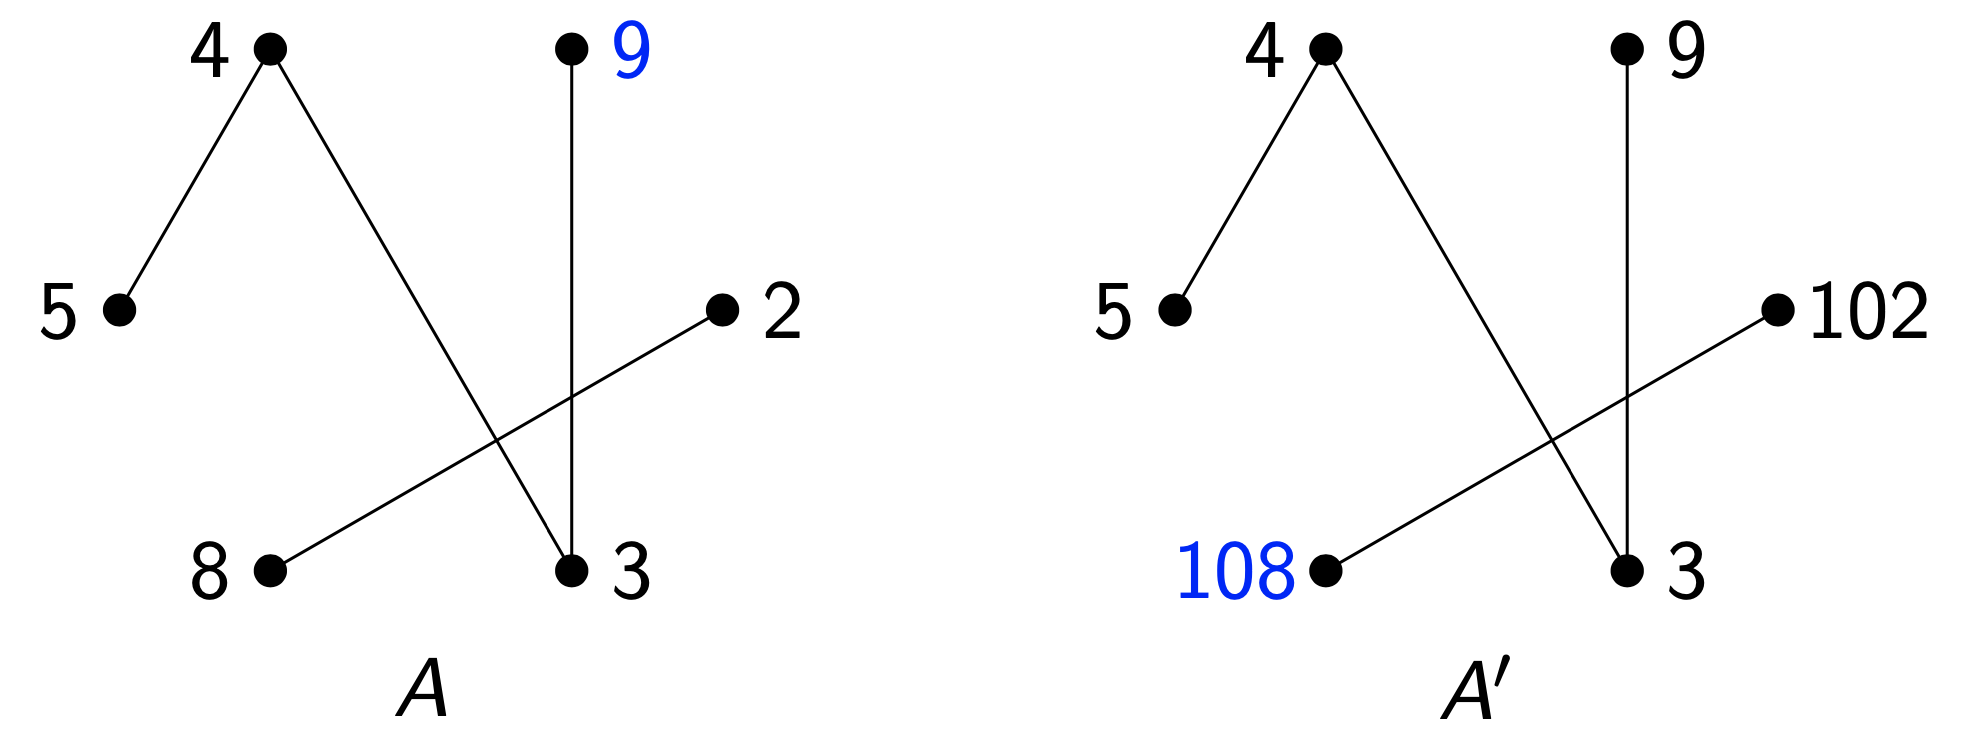
\includegraphics[width=0.9\linewidth]{cs3230-maximum-problem-graph.png} 

    $M$ cannot differentiate $A$ and $A'$.
  \end{niceproof}

  \subsubsection{Second Largest Problem}

  \textit{problem}: find the second largest element in $<2n-3$ comparisons (2x Maximum $\Rightarrow$ $\scriptstyle (n-1) + ((n-1)-1) = 2n-3$ )

  \begin{itemize}
    \item \textit{solution}: \textbf{knockout tournament} $\Rightarrow n + \lceil \lg n \rceil - 2$
      \\* 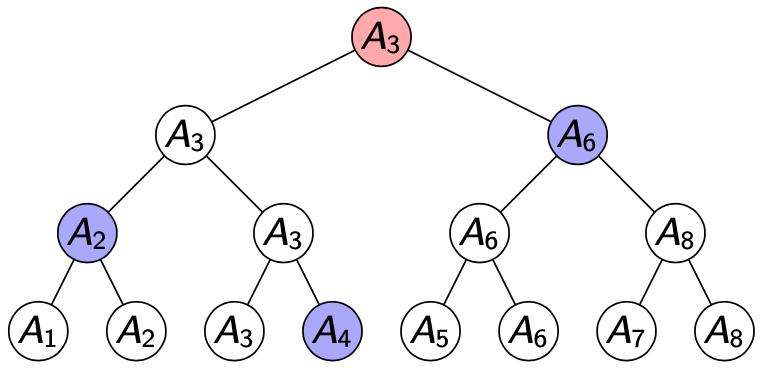
\includegraphics[width=0.8\linewidth]{cs3230-second-largest-solution.png} 
      \begin{enumerate}
        \item bracket system: $n-1$ matches 
          \begin{itemize}
            \item every non-winner has lost exactly once
          \end{itemize}
        \item then compare the elements that have lost to the largest
          \begin{itemize}
            \item the 2nd largest element must have lost to the winner
            \item compares $\lceil \lg n \rceil$ elements that have lost to the winner using $\lceil \lg n \rceil -1$ comparisons 
          \end{itemize}
      \end{enumerate}
  \end{itemize}

  \subsubsection{Sorting}

  \textit{Claim.} there is a sorting algorithm that requires $\leq n \lg n - n + 1$ comparisons.

  \begin{niceproof}
    every sorting algorithm must make $\geq \lg (n!)$ comparisons.
  \end{niceproof}

  \begin{enumerate}
    \item let set $\mathcal{U}$ be the set of all permutations of the set $\{1, \dots, n\}$ that the adversary could choose as array $A$. $\vert \mathcal{U} \vert = n!$ 
    \item for each query "is $A_i > A_j$?", 
      \\* if $\mathcal{U}_{yes} = \{A \in \mathcal{U} : A_i > A_j\}$ is of size $\geq \vert\mathcal{U}\vert /2$, set $\mathcal{U} := \mathcal{U}_{yes}$. else: $\mathcal{U} := \mathcal{U} \backslash \mathcal{U}_{yes}$
    \item the size of $\mathcal{U}$ decreases by at most half with each comparison
    \item with $< \lg (n!)$ comparisons, $\mathcal{U}$ will still contain at least 2 permutations
  \end{enumerate}

  \begin{tightcenter}
    $n! \geq (\frac{n}{e})^n$ 
    \\* $\Rightarrow \lg (n!) \geq n \lg (\frac{n}{e}) = n \lg n - n \lg e$
    \\* $\approx n \lg n - 1.44n$
    \\* $\Rightarrow$ roughly $n \lg n$ comparisons are \textbf{required} and \textbf{sufficient} for sorting $n$ numbers
  \end{tightcenter}

  \subsection{String Model}

  \begin{tightcenter}
    \begin{tabular}{|c|l|}
      \hline
      input & string of $n$ bits \\\hline
      each query & find out \textbf{one bit} of the string \\ \hline
    \end{tabular}
  \end{tightcenter}

  \begin{itemize}
    \item $n$ queries are \textbf{necessary} and \textbf{sufficient} to check if the input string is all 0s.
    \item \definition{query complexity} number of bits of the input string queried by the algorithm
    \item \definition{evasive} a problem requiring $n$ query complexity
  \end{itemize}

  \subsection{Graph Model}

  \begin{tightcenter}
    \begin{tabular}{|c|p{0.7\linewidth}|}
      \hline
      input & (symmetric) adjacency matrix of an $n$-node undirected graph \\\hline
      each query & find out if an edge is present between two chosen nodes (one entry of $G$) \\\hline
    \end{tabular}
  \end{tightcenter}

  \begin{itemize}
    \item \definition{evasive} requires $\binom{n}{2}$ queries
    \item \textit{Proof}. determining whether the graph is connected is evasive (requires $\binom{n}{2}$ queries) 
      \begin{enumerate}
        \item suppose $M$ is an algorithm making $\leq \binom{n}{2}$ queries.
        \item whenever $M$ makes a query, the algorithm tries not adding this edge, but adding all remaining unqueried edges. 
          \begin{enumerate}
            \item if the resulting graph is connected, $M$ replies $0$ (i.e. edge does not exist)
            \item else: replies $1$ (edge exists)
          \end{enumerate}
        \item after $< \binom{n}{2}$ queries, at least one entry of the adjacency matrix is unqueried.
      \end{enumerate}
      \qed
  \end{itemize}


  \section{02. ASYMPTOTIC ANALYSIS}

  \begin{itemize}
    \item \definition{algorithm} a \textit{finite} sequence of well-defined instructions to solve a given computational problem
    \item \definition{word-RAM model} runtime is the total number of instructions executed
      \begin{itemize}
        \item operators, comparisons, if, return, etc
        \item each instruction operates on a \textit{word} of data (limited size) $\Rightarrow$ fixed constant amount of time
      \end{itemize}

  \end{itemize}

  \subsection{Asymptotic Notations}

  \begin{tightcenter}
    \textbf{upper bound ($\leq$)}: $f(n) = O(g(n))$
    \\* if $\exists c>0, n_0>0$ such that $\forall n \geq n_0$, 
    \begin{tightbox}
      $0 \leq f(n) \leq cg(n)$
    \end{tightbox}

    \ \\ \textbf{lower bound ($\geq$)}: $f(n) = \Omega(g(n))$
    \\* if $\exists c>0, n_0>0$ such that $\forall n \geq n_0$, 
    \begin{tightbox}
      $0 \leq cg(n) \leq f(n)$
    \end{tightbox}

    \ \\ \textbf{tight bound}: $f(n) = \Theta(g(n))$
    \\* if $\exists c_1, c_2, n_0>0$ such that $\forall n \geq n_0,$
    \begin{tightbox}
      $0 \leq c_1 g(n) \leq f(n) \leq c_2 g(n)$ 
    \end{tightbox}

    \ \\ \textbf{$o$-notation ($<$)}: $f(n) = o(g(n))$
    \\* if $\forall c>0, \exists n_0>0$ such that $\forall n \geq n_0$, 
    \begin{tightbox}
      $0 \leq f(n) < cg(n)$
    \end{tightbox}

    \ \\ \textbf{$\omega$-notation ($>$)}: $f(n) = \omega(g(n))$
    \\* if $\forall c>0, \exists n_0>0$ such that $\forall n \geq n_0$, 
    \begin{tightbox}
      $0 \leq cg(n) < f(n)$
    \end{tightbox}
  \end{tightcenter}

  \subsection{Limits}

  Assume $f(n), g(n) > 0$.
  \begin{align*}
    &\lim\limits_{n \to \infty} \frac{f(n)}{g(n)} = 0 &\Rightarrow f(n) = o(g(n)) \\
    &\lim\limits_{n \to \infty} \frac{f(n)}{g(n)} < \infty &\Rightarrow f(n) = O(g(n)) \\
    0 < &\lim\limits_{n \to \infty} \frac{f(n)}{g(n)} < \infty &\Rightarrow f(n) = \Theta(g(n)) \\
        &\lim\limits_{n \to \infty} \frac{f(n)}{g(n)} > 0 &\Rightarrow f(n) = \Omega(g(n)) \\
        &\lim\limits_{n \to \infty} \frac{f(n)}{g(n)} = \infty &\Rightarrow f(n) = \omega(g(n))
  \end{align*}

  \begin{niceproof}
    using delta epsilon definition
  \end{niceproof}

  \subsection{Properties of Big O}

  \begin{fixedbox}
    $\Theta(g(n)) = O(g(n)) \cap \Omega(g(n))$
  \end{fixedbox}

  \begin{itemize}
    \item \textbf{transitivity} - applies for $O, \Theta, \Omega, o, \omega$
      $f(n) = O(g(n)) \land g(n) = O(h(n)) \Rightarrow f(n) = O(h(n))$ 
    \item \textbf{reflexivity} - for $O, \Omega, \Theta, \quad f(n) = O(f(n))$ 
    \item \textbf{symmetry} - $f(n) = \Theta(g(n)) \iff g(n) = \Theta(f(n))$
    \item \textbf{complementarity} - 
      \begin{itemize}
        \item $f(n) = O(g(n)) \iff g(n) = \Omega(f(n))$
        \item $f(n) = o(g(n)) \iff g(n) = \omega(f(n))$
      \end{itemize}
    \item \textbf{misc}
      \begin{itemize}
        \item if $f(n) = \omega(g(n))$, then $f(n) = \Omega(g(n))$
        \item if $f(n) = o(g(n))$, then $f(n) = O(g(n))$
      \end{itemize}
  \end{itemize}

  \begin{fixedbox}[0.8]
    $\log\log n < \log n < (\log n)^k < n^k < k^n$
  \end{fixedbox}

  insertion sort: $O(n^2)$ with worst case $\Theta(n^2)$

  \section{03. ITERATION, RECURSION, DIVIDE-AND-CONQUER}

  \subsection{Iterative Algorithms}

  \begin{itemize}
    \item \definition{iterative} loop(s), sequentially processing input elements
    \item \textbf{loop invariant} implies correctness if 
      \begin{itemize}
        \item \textit{initialisation} - true before the first iteration of the loop
        \item \textit{maintenance} - if true before an iteration, it remains true at the beginning of the next iteration
        \item \textit{termination} - true when the algorithm terminates
      \end{itemize}
  \end{itemize}

  \subsubsection{examples}

  \begin{itemize}
    \item \textbf{insertionSort}: with loop variable as $j$, $A[1..J-1]$ is sorted.
    \item \textbf{selectionSort}: with loop variable as $j$, the array $A[1..j-1]$ is sorted and contains the $j-1$ smallest elements of $A$.
    \item \textbf{Misra-Gries algorithm} (determines which bit occurs more in an $n$-bit array $A$):
      \begin{itemize}
        \item if there is an equal number of 0's and 1's, then $id=\bot$ and $count = 0$
        \item if $z \in \{0, 1\}$ is the majority element, then $id=z$ and $count$ equals the difference between the count of the bits.
      \end{itemize}
  \end{itemize}


  \subsection{Divide-and-Conquer}

  \subsubsection{powering a number}

  \textit{problem:} compute $f(n, m) = a^n\Mod{m}$ for all $n, m \in \mathbb{Z}$

  \begin{itemize}
    \item observation: $f(x+y, m) = f(x, m) * f(y, m) \Mod{m}$
    \item \textbf{naive solution}: recursively compute and combine $f(n-1, m) * f(1, m) \Mod m$ 
      \begin{itemize}
        \item $T(n) = T(n-1) + T(1) + \Theta(1) \Rightarrow T(n) = \Theta (n)$
      \end{itemize}
    \item \textbf{better solution}: divide and conquer
      \begin{itemize}
        \item divide: trivial
        \item conquer: recursively compute $f(\lfloor n / 2 \rfloor, m)$ 
        \item combine: 
          \begin{itemize}
            \item $f(n, m) = f(\lfloor n / 2 \rfloor, m)^2 \Mod m$ if n is even
            \item $f(n, m) = f(1, m) * f(\lfloor n / 2 \rfloor, m)^2 \Mod m$ if odd
          \end{itemize}
        \item $T(n) = T(n/2) + \Theta(1) \Rightarrow \Theta(\log n)$
      \end{itemize}
  \end{itemize}

  \section{Solving Recurrences}

  for $a$ sub-problems of size $\frac{n}{b}$ where $f(n)$ is the time to divide and combine, 
  \begin{tightcenter}
    $T(n) = aT(\frac{n}{b}) + f(n)$
  \end{tightcenter}

  \subsection{Recursion tree}

  total = height $\times$ number of leaves

  \begin{itemize}
    \item each node represents the cost of a single subproblem
    \item height of the tree = longest path from root to leaf
  \end{itemize}

  \begin{tightcenter}
    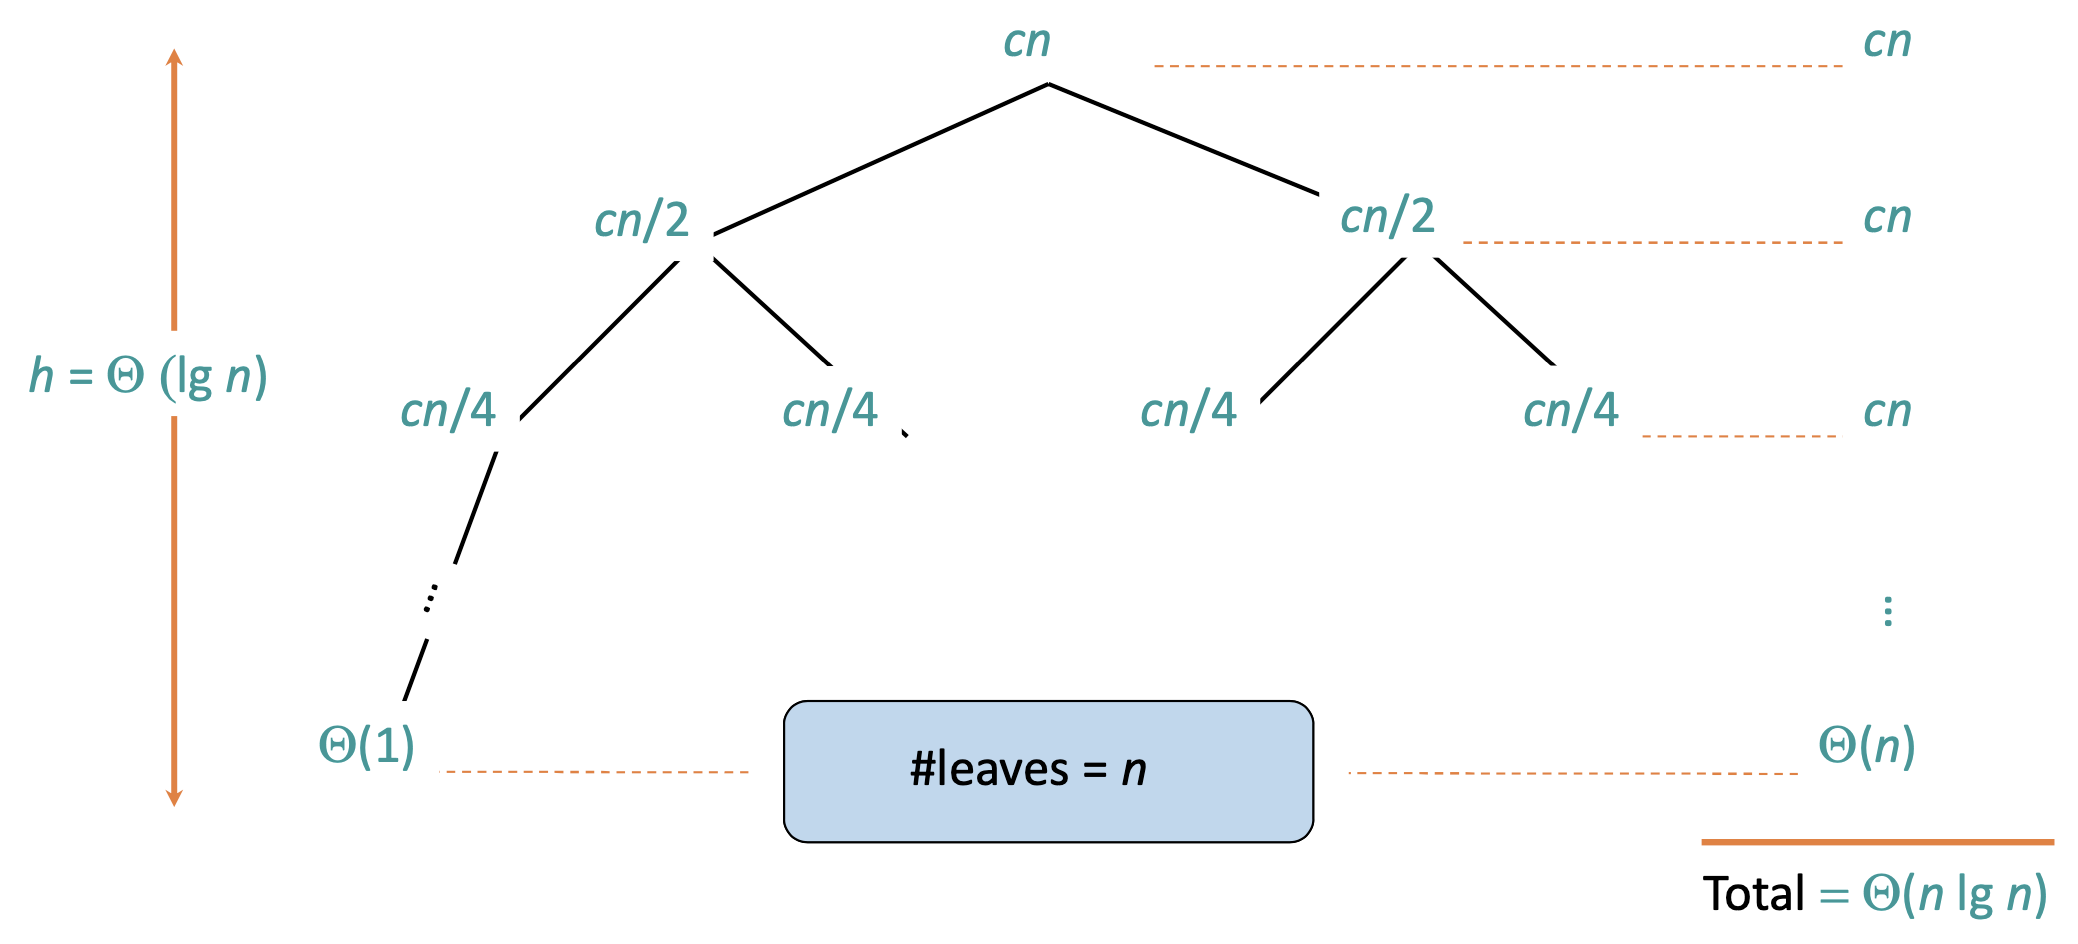
\includegraphics[width=0.9\linewidth]{cs3230-recursion-tree-example-1.png} 
    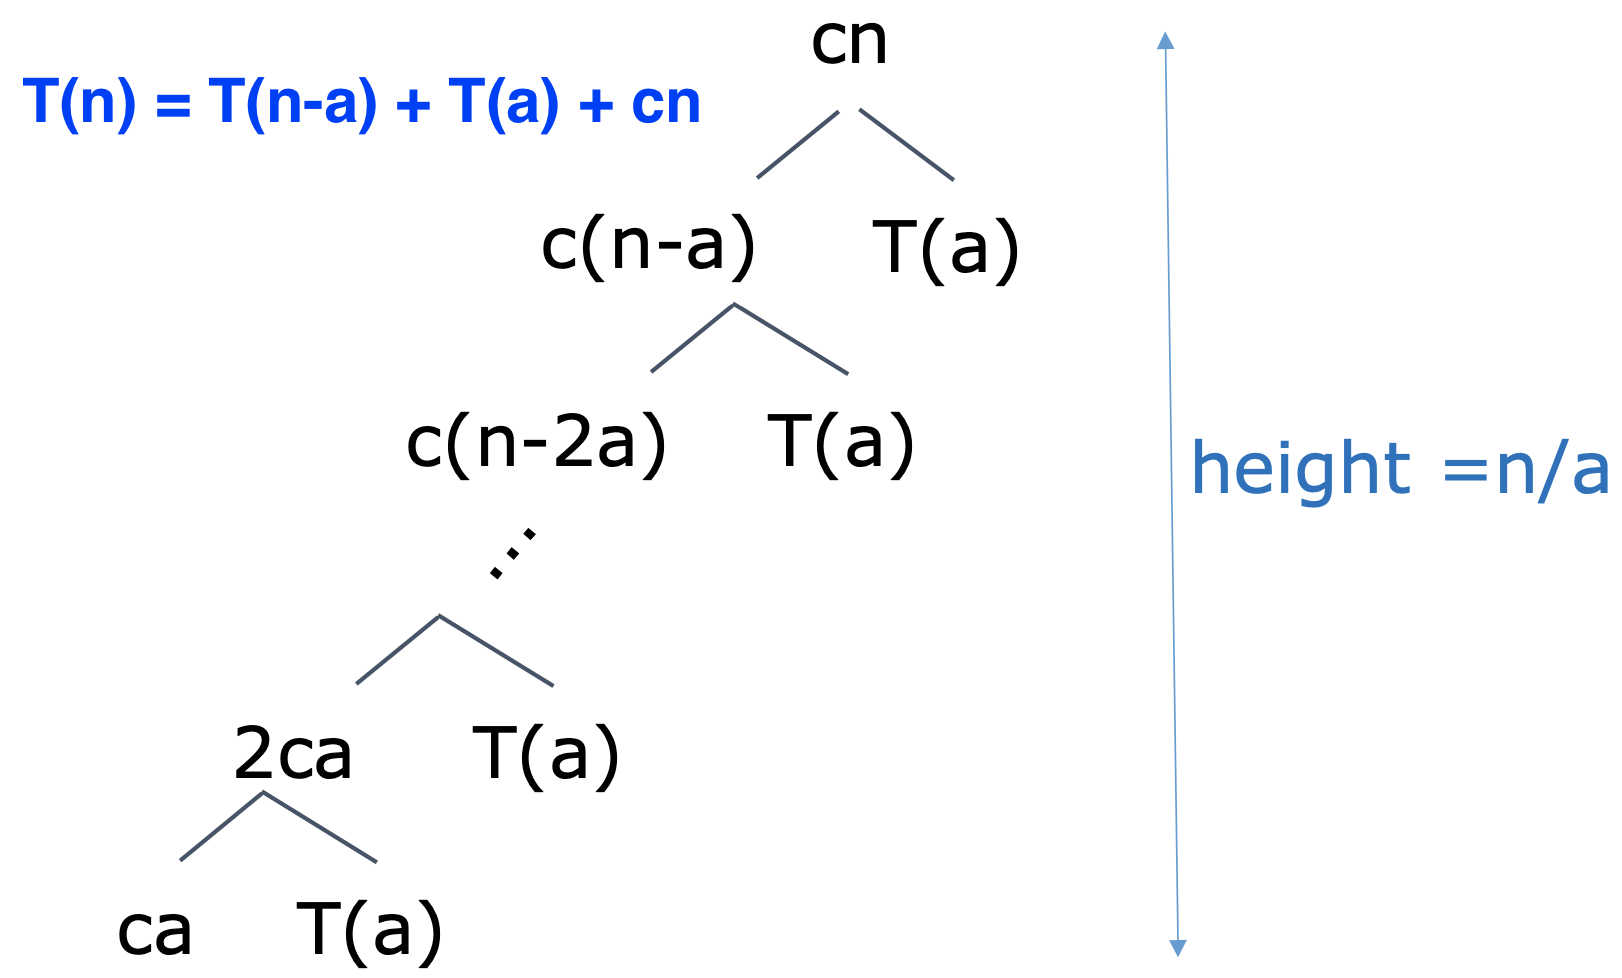
\includegraphics[width=0.6\linewidth]{cs3230-recursion-tree-example-2.png} 
  \end{tightcenter}

  \subsection{Master method}

  $a \geq 1, b > 1,$ and $f$ is asymptotically positive

  \begin{math}
    T(n) = aT(\frac{n}{b}) + f(n) = \begin{cases}
      \Theta(n^{\log_ba}) & \text{ if } f(n) < n^{\log_ba} \text{ polynomially}
      \\ \Theta(n^{\log_ba} \log n) & \text{ if } f(n) = n^{\log_ba} 
      \\ \Theta(f(n)) & \text{ if } f(n) > n^{\log_ba} \text{ polynomially}
    \end{cases}
  \end{math}

  \subsubsection{three common cases}

  \begin{enumerate}
    \item If $f(n) = O(n^{\log_b a-\epsilon})$ for some constant  $\epsilon > 0$, 
      \begin{itemize}
        \item $f(n)$ grows polynomially slower than $n^{\log_ba}$ by $n^\epsilon$ factor.
        \item then $T(n) = \Theta(n^{\log_ba})$.
      \end{itemize}
    \item If $f(n) = \Theta(n^{\log_ba} \log^kn) $ for some $k \geq 0$,
      \begin{itemize}
        \item $f(n)$ and $n^{\log_ba}$ grow at similar rates.
        \item then $T(n) = \Theta(n^{\log_ba}\log n)$
      \end{itemize}
    \item If $f(n) = \Omega(n^{\log_ba + \epsilon})$ for some constant $\epsilon > 0$, 
      \begin{itemize}
        \item and $f(n)$ satisfies the \textbf{regularity condition} 
          \begin{itemize}
            \item $af(n/b) \leq cf(n)$ for some constant $c<1$ and \\* all sufficiently large $n$, 
            \item this guarantees that the sum of subproblems is smaller than $f(n)$.
          \end{itemize} 
        \item $f(n)$ grows polynomially faster than $n^{\log_ba}$ by $n^\epsilon$ factor
        \item then $T(n) = \Theta(f(n))$.
      \end{itemize}
  \end{enumerate}

  \subsection{Substitution method}

  \begin{enumerate}
    \item guess that $T(n) = O(f(n))$. 
    \item verify by induction:
      \begin{enumerate}
        \item to show that for $n \geq n_0$, $T(n) \leq c \cdot f(n)$
        \item set $c = \max\{2, q\}$ and $n_0 = 1$
        \item verify base case(s): $T(n_0) = q$
        \item recursive case ($n > n_0$):
          \begin{itemize}
            \item by strong induction, assume $T(k) \leq c \cdot f(k)$ for $n > k \geq n_0$
            \item T(n) = <recurrence> ... $\leq c \cdot f(n)$
          \end{itemize}
        \item hence $T(n) = O(f(n))$.
      \end{enumerate}
  \end{enumerate}
  \attention may not be a tight bound!

  \subsubsection{example}

  \begin{niceproof}
    $T(n) = 4T(n/2) + n^2/\lg n \Rightarrow \Theta(n^2\lg \lg n)$

    $T(n) = 4T(n/2) + \frac{n^2}{\lg n}$ \\
    $= 4( 4T(n/4) + \frac{(n/2)^2}{\lg n - lg 2} ) + \frac{n^2}{\lg n}$ \\ 
    $= 16 T(n/4) + \frac{n^2}{\lg n - \lg 2} + \frac{n^2}{\lg n}$ \\
    $= \sum\limits^{\lg n}_{k=1} \frac{n^2}{\lg n - k}$ \\
    $= n^2 \lg \lg n$ by approx. of harmonic series ($\sum\frac{1}{k}$)
  \end{niceproof}

  \begin{niceproof}
    $T(n) = 4T(n/2) + n \Rightarrow O(n^2)$

    To show that for all $n \geq n_0$, $T(n) \leq c_1n^2 - c_2n$

    1. Set $c_1 = q+1, c_2 = 1, n_0 = 1$. 

    2. Base case ($n=1$): subbing into $c_1n^2 - c_2n$,
    $T(1) = q \leq (q+1)(1)^2 - (1)(1)$ 

    3. Recursive case ($n>1$):
    \begin{itemize}
      \item by strong induction, assume $T(k) \leq c_1 \cdot k^2 - c_2 \cdot k$ for all $n>k \geq 1$ 
      \item $T(n) = 4T(n/2) + n$ 
        \\* $\quad\quad = 4(c_1 (n/2)^2 - c_2 (n/2)) + n$
        \\* $\quad\quad = c_1n^2 - 2c_2n + n $
        \\* $\quad\quad = c_1n^2 - c_2n + (1-c_2) n$
        \\* $\quad\quad = c_1n^2 - c_2n \quad $ since $c_2=1 \Rightarrow 1-c_2 = 0$
        \\* \qed
    \end{itemize}
  \end{niceproof}

  \section{04. AVERAGE-CASE ANALYSIS \& RANDOMISED ALGORITHMS}

  \begin{itemize}
    \item \definition[$A(n)$]{average case} expected running time when the input is chosen uniformly at random from the set of all $n!$ permutations
      \begin{itemize}
        \item $A(n) = \frac{1}{n!} \sum_\pi Q(\pi)$ where $Q(\pi)$ is the time complexity when the input is permutation $\pi$.
        \item $A(n) = \mathop{\mathbb{E}}\limits_{x \sim \mathcal{D}_n} [ \text{Runtime of Alg on }x ] $
          \begin{itemize}
            \item $ \mathbb{E}_{x \sim \mathcal{D}_n} $ is a probability distribution on $U$ restricted to inputs of size $n$.
          \end{itemize}
      \end{itemize}
  \end{itemize}

  \subsection{Quicksort Analysis}

  \begin{itemize}
    \item divide \& conquer, linear-time $\Theta(n)$ partitioning subroutine
    \item assume we select the first array element as pivot 
    \item $T(n) = T(j) + T(n-j-1) + \Theta(n)$
      \begin{itemize}
        \item if the pivot produces subarrays of size $j$ and $(n-j-1)$
      \end{itemize}
    \item \textbf{worst-case}: $T(n) = T(0) + T(n-1) + \Theta(n) \Rightarrow \Theta(n^2)$ 
  \end{itemize}

  \begin{niceproof}
    for quicksort, $A(n) = O(n \log n)$

    let $P(i)$ be the set of all those permutations of elements $\{e_1, e_2, \dots, e_n\}$ that begins with $e_i$.

    Let $G(n, i)$ be the average running time of quicksort over $P(i)$.
    Then $G(n) = A(i-1) + A(n-i) + (n-1)$.
    $A(n) = \frac{1}{n} \sum_{i=1}^n G(n, i)$
    \\ $\quad\quad = \frac{1}{n} \sum_{i=1}^n ( A(i-1) + A(n-i) + (n-1) )$
    \\ $\quad\quad = \frac{2}{n} \sum_{i=1}^n A(i-1)+n-1$
    \\ $\quad\quad = O(n\log n)$ by taking it as area under integration
  \end{niceproof}

  \subsubsection{quicksort vs mergesort}

  \begin{center}
    \begin{tabular}{|c|c|c|c|}
      \hline
      & average & best & worst \\\hline
      quicksort & $1.39n\lg n$ &  $n \lg n$ & $n(n-1)$ \\\hline
      mergesort & $n\lg n$ &  $n \lg n$ & $n \lg n$ \\\hline
    \end{tabular}
  \end{center}

  \begin{itemize}
    \item disadvantages of mergesort:
      \begin{itemize}
        \item overhead of temporary storage
        \item cache misses
      \end{itemize}
    \item advantages of quicksort
      \begin{itemize}
        \item in place
        \item reliable (as $n \uparrow$, chances of deviation from avg case $\downarrow$)
      \end{itemize}
    \item issues with quicksort
      \begin{itemize}
        \item \definition{distribution-sensitive} time taken depends on the initial (input) permutation
      \end{itemize}
  \end{itemize}

  \subsection{Randomised Algorithms}

  \begin{itemize}
    \item \definition{randomised algorithms} output and running time are \textbf{functions} of the \textbf{input} and \textbf{random bits chosen}
      \begin{itemize}
        \item vs non-randomised: output \& running time are functions of the \textit{input only}
      \end{itemize}
    \item expected running time = worst-case running time = 
      \\* $E(n) = \max\limits_{ \text{input $x$ of size $n$} } \mathbb{E} [ \text{Runtime of RandAlg on }x ] $
    \item \textbf{randomised quicksort}: choose pivot at random 
      \begin{itemize}
        \item probability that the runtime of \textit{randomised} quicksort exceeds average by $x\% = n^{-\frac{x}{100}\ln\ln n}$ 
        \item P(time takes at least double of the average) = $10^{-15}$
        \item distribution insensitive
      \end{itemize}
  \end{itemize}

  \subsubsection{Randomised Quicksort Analysis}

  $T(n) = n-1 + T(q-1) + T(n-q)$

  Let $A(n) = \mathbb{E}[T(n)]$ where the expectation is over the randomness in expectation.

  Taking expectations and applying linearity of expectation:
  $A(n) = n-1 + \frac{1}{n} \sum^n_{q=1} (A(q-1) + A(n-q)) $ 
  $\;\quad\quad = n-1 + \frac{2}{n} \sum\limits^{n-1}_{q=1} A(q) $ 

  $A(n) = n \log n \quad \Rightarrow$ same as average case quicksort

  \subsubsection{Randomised Quickselect}

  \begin{itemize}
    \item $O(n)$ to find the $k^{th}$ smallest element
    \item randomisation: unlikely to keep getting a bad split
  \end{itemize}

  \subsubsection{Types of Randomised Algorithms}

  \begin{itemize}
    \item randomised \textbf{Las Vegas} algorithms
      \begin{itemize}
        \item output is always correct
        \item runtime is a \textit{random variable} 
        \item e.g. randomised quicksort, randomised quickselect
      \end{itemize}
    \item randomised \textbf{Monte Carlo} algorithms
      \begin{itemize}
        \item output may be incorrect with some small probability
        \item runtime is \textit{deterministic}
      \end{itemize}
  \end{itemize}

  \textbf{examples}
  \begin{itemize}
    \item \textit{smallest enclosing circle:} given $n$ points in a plane, compute the smallest radius circle that encloses all $n$ points
      \begin{itemize}
        \item best \textbf{deterministic} algorithm: $O(n)$, but complex
        \item las vegas: average $O(n) $, simple solution
      \end{itemize}
    \item \textit{minimum cut:} given a connected graph $G$ with $n$ vertices and $m$ edges, compute the smallest set of edges whose removal would disconnect $G$.
      \begin{itemize}
        \item best \textbf{deterministic} algorithm: $O(mn)$
        \item \textbf{monte carlo}: $O(m \log n) $, error probability $n^{-c}$ for any $c$
      \end{itemize}
    \item \textit{primality testing:} determine if an $n$ bit integer is prime
      \begin{itemize}
        \item best \textbf{deterministic} algorithm: $O(n^6)$
        \item \textbf{monte carlo}: $O(kn^2)$, error probability $2^{-k}$ for any $k$
      \end{itemize}
  \end{itemize}

  \subsection{Geometric Distribution}

  Let $X$ be the number of trials repeated until success. 

  $X$ is a random variable and follows a geometric distribution with probability $p$.

  \begin{tightcenter}
    Expected number of trials, $E[X] = \frac{1}{p} $
    \\* $ Pr[X=k] = q^{k-1}p $
  \end{tightcenter}

  \subsubsection{Linearity of Expectation}

  For any two events $ X, Y $ and a constant $ a $, 
  \begin{tightcenter}
    $ E[X+Y] = E[X] + E[Y] $
    \\ $ E[aX] = aE[X] $
  \end{tightcenter}

  \subsubsection{Coupon Collector Problem}

  \textit{$ n $ types of coupon are put into a box and randomly drawn with replacement.
  What is the expected number of draws needed to collect at least one of each type of coupon?}

  \begin{itemize}
    \item let $ T_i $ be the time to collect the $ i $-th coupon after the $ i-1 $ coupon has been collected. 
      \begin{itemize}
        \item Probability of collecting a new coupon, $ p_i = \frac{(n-(i-1))}{n}  $
        \item $ T_i $ has a \textbf{geometric distribution}
        \item $ E[T_i] = 1/p_i $
      \end{itemize}
    \item total number of draws, $ T = \sum\limits^n_{i=1} T_i $
    \item $ E[T] = E[\sum\limits^n_{i=1}T_i] = \sum\limits^n_{i=1}E[T_i] $ by linearity of expectation
      \\* $ = \sum\limits^n_{i=1} \frac{n}{n-(i-1)} = n \cdot \sum\limits^n_{i=1} \frac{1}{i} = \Theta(n \lg n) $
  \end{itemize}

  \section{05. HASHING}

  \subsection{Dictionary ADT}

  \begin{itemize}
    \item different types:
      \begin{itemize}
        \item \textbf{static} - fixed set of inserted items; only care about queries
        \item \textbf{insertion-only} - only insertions and queries
        \item \textbf{dynamic} - insertions, deletions, queries
      \end{itemize}
    \item implementations
      \begin{itemize}
        \item sorted list (static) - $O(\log N)$ query
        \item balanced search tree (dynamic) - $O(\log N)$ all operations
        \item direct access table
          \begin{itemize}
            \item $\times$ needs items to be represented as non-negative integers (\textbf{prehashing})
            \item $\times$ huge space requirement
          \end{itemize}
      \end{itemize}
    \item using $\mathcal{H}$ for dictionaries: need to store both the hash table and the matrix $A$.
      \begin{itemize}
        \item additional storage overhead $= \Theta(\log N \cdot \log \vert U \vert)$, if $M = \Theta(N)$
        \item other universal hashing constructions may have more efficient hash function evaluation
      \end{itemize}
    \item \textit{associative array} - has both key and value (dictionary in this context has only key)
  \end{itemize}

  \subsection{Hashing}

  \begin{itemize}
    \item \ildefinition{hash function}, $h:U \to \{1, \dots, M\}$ gives the location of where to store in the hash table
      \begin{itemize}
        \item notation: $[M] = \{ 1, \dots, M \}[M] = \{ 1, \dots, M \}$
        \item storing $N$ items in hash table of size $M$
      \end{itemize}
    \item \definition{collision} for two different keys $x$ and $y$, $h(x) = h(y)$ 
      \begin{itemize}
        \item resolve by \textbf{chaining}, \textbf{open addressing}, etc
      \end{itemize}
    \item desired properties 
      \begin{itemize}
        \item $\checkmark$ minimise collisions - \code{query(x)} and \code{delete(x)} take time $\Theta(\vert h(x) \vert)$
        \item $\checkmark$ minimise storage space - aim to have $M = O(N)$
        \item $\checkmark$ function $h$ is easy to compute (assume constant time)
      \end{itemize}
    \item if $\vert U \vert \geq (N-1) M + 1$, for any $h:U \to [M]$, there is a set of $N$ elements having the same hash value.
      \begin{itemize}
        \item \textit{Proof}: pigeonhole principle
      \end{itemize}
    \item use \textbf{randomisation} to overcome the adversary
      \begin{itemize}
        \item e.g. randomly choose between two \textit{deterministic} hash functions $h_1$ and $h_2$ 
          \\* $\Rightarrow$ for any pair of keys, with probability $\geq \frac{1}{2} $, there will be no collision
      \end{itemize}
  \end{itemize}

  \subsection{Universal Hashing}

  Suppose $\mathcal{H}$ is a set of hash functions mapping $U$ to $[M]$. 

  \begin{tightcenter}
    $\mathcal{H}$ is \ildefinition{universal} if $\forall \, x \neq y$,
    $\frac{\vert h \in \mathcal{H}: h(x) = h(y) \vert}{\vert H \vert} \leq \frac{1}{M} $
    \\* or $\mathop{Pr}\limits_{h \sim \mathcal{H}} [h(x) = h(y)] \leq \frac{1}{M}$
  \end{tightcenter}
  \begin{itemize}
    \item aka: for any $x \neq y$, if $h$ is chosen uniformly at random from a universal $\mathcal{H}$, then there is at most $ \frac{1}{M} $ probability that $h(x) = h(y)$
    \item probability where $h$ is sampled uniformly from $\mathcal{H}$
    \item aka: for any $x\neq y$, the fraction of hash functions with collisions is at most $\frac{1}{M}$.
  \end{itemize}

  \subsubsection{Properties of universal hashing}

  \textbf{Collision Analysis}

  \begin{itemize}
    \item for any $N$ elements $x_1, \dots, x_N \in \mathcal{U}$, the \textbf{expected number of collisions} between  $x_N$ and other elements is $<N/M$.
      \begin{itemize}
        \item it follows that for $K$ operations, the expected cost of the last operation is $< K/M = O(1)$ if $M>K$.
      \end{itemize}
      \begin{niceproof}
        by definition of Universal Hashing, each element  $x_1, \dots, x_{N-1} \in \mathcal{U}$ has at most $\frac{1}{M}$ probability of collision with $x_N$ (over random choice of $h$).

        by indicator r.v., $\scriptstyle E[A_i] = P(A_i = 1) \leq \frac{1}{M}$.
        expected number of collisions = $(N-1) \cdot \frac{1}{M} < \frac{N}{M}$.
      \end{niceproof}

    \item if $x_1, \dots, x_N$ are added to the hash table, and $M>N$, the expected \textbf{number of pairs} $(i, j)$ with collisions is $<2N$.

      \begin{niceproof}
        let $A_{ij}$ be an indicator r.v. for collision. 
        \\* $ \mathbb{E} [\sum\limits_{1 \leq i, j \leq N} A_{ij}] = \sum\limits^N_{i=1} \mathbb{E}[A_{ii}] + \sum\limits_{i \neq j} \mathbb{E} [A_{ij}] $
        \\* $\quad\quad \leq N \cdot 1 + N(N-1) \cdot \frac{1}{M} < 2N $
      \end{niceproof}
  \end{itemize}

  \textbf{Expected Cost}

  \begin{itemize}
    \item for any sequence of $N$ operations, if $M > N$, then the \textbf{expected total cost} for executing the sequence is $O(N)$.
      \begin{niceproof}
        linearity of expectation; sum up expected costs
      \end{niceproof}
  \end{itemize}

  \subsubsection{Construction of Universal Family}

  \textit{Obtain a universal family of hash functions with $M = O(N)$.}

  \begin{itemize}
    \item Suppose $U$ is indexed by $u$-bit strings and $M = 2^m$. 
    \item For any $m \times u$ binary matrix $A$, \ildefinition{$h_A(x) = Ax \Mod 2$ }
      \begin{itemize}
        \item each element \code{x => x \% 2}
        \item $x$ is a $u \times 1$ matrix $\Rightarrow Ax$ is $m \times 1$
      \end{itemize}
    \item \textit{Claim}: $\{h_A:A \in \{0, 1\}^{m \times u}\}$ is universal
    \item e.g. $U = \{00, 01, 10, 11\}, M = 2$ 
      \begin{itemize}
        \item $h_{ab}$ means $A = [a\; b]$
          \\* {\rowcolors{2}{gray!15}{gray!5}\begin{tabular}
              {ccccc}
              \rowcolor{cyan!10} 
              \hline
              \, & 00 & 01 & 10 & 11 \\\hline
              $h_{00}$ & 0 & 0 & 0 & 0 \\
              $h_{01}$ & 0 & 1 & 0 & 1 \\
              $h_{10}$ & 0 & 0 & 1 & 1 \\
              $h_{11}$ & 0 & 1 & 1 & 0 \\\hline
            \end{tabular}
          }
      \end{itemize}
  \end{itemize}

  \begin{niceproof}
    Let $x \neq y$. Let $z = x - y$. We know $z \neq 0$. 

    Collision: $\scriptstyle P(Ax = Ay) = P[A(x-y) = 0] = P(Az = 0)$.

    To show $P(Az = 0) \leq \frac{1}{M} $.

    \textit{Special case} - Suppose $z$ is $1$ at the $i$-th coordinate but 0 everywhere else. Then $Az$ is the $i$-th column of $A$.
    Since the $i$-th column is uniformly random, $P(Az = 0) = \frac{1}{2^m} = \frac{1}{M} $.

    \textit{General case} - Suppose $z$ is $1$ at the $i$-th coordinate. Let $z = [z_1 \; z_2 \; \dots \; z_u]^T$. 
    $A = [A_1 \; A_2 \; \dots \; A_u] \quad$ hence $A_k$ is the $k$-th column of $A$.
    \\* Then $Az = z_1 A_1 + z_2 A_2 + \dots + z_u A_u$.
    \\* $Az = 0 \Rightarrow z_1 A_1 = -(z_2 A_2 + \dots + z_u A_u) \quad(*)$
    \\* We fix $z_1A_1$ to be an arbitrary $m \times 1$ matrix of 1s and 0s. The probability that $(*)$ holds is $ \frac{1}{2^m} $.
  \end{niceproof}

  \subsection{Perfect Hashing}

  \textbf{static case} - $N$ fixed items in the dictionary $x_1, x_2, \dots, x_N$

  \textit{To perform \texttt{Query} in $O(1)$ worst-case time.}

  \subsubsection{Quadratic Space: $M=N^2$}

  if $\mathcal{H}$ is universal and $M = N^2$, and $h$ is sampled uniformly from $\mathcal{H}$, then the expected number of collisions is $<1$.

  \begin{niceproof}
    for $i \neq j$, let indicator r.v. $A_{ij}$ be equal to $1$ if $h(x_i) = h(x_j)$, or $0$ otherwise.

    By universality, $E[A_{ij}] = P(A_{ij} = 1) \leq 1/N^2$

    $E[ \text{\# collisions}] = \sum\limits_{i < j} E[A_{ij}] \leq \binom{N}{2} \frac{1}{N^2} <1$
  \end{niceproof}

  It follows that there exists $h \in \mathcal{H}$ causing no collisions (because if not, $\mathbb{E}$[\#collisions] would be $\geq 1$).

  \subsubsection{2-Level Scheme: $M=N$}

  \begin{itemize}
    \item No collision and less space needed
  \end{itemize}

  \textbf{Construction}

  Choose $h:U \to [N]$ from a universal hash family.

  \begin{itemize}
    \item Let $L_k$ be the number of $x_i$'s for which $h(x_i) = k$. 
    \item Choose  $h_1, \dots, h_N$ \textbf{second-level} hash functions $h_k: [N] \to [(L_k)^2]$ s.t. there are no collisions among the $L_k$ elements mapped to $k$ by $h$.
      \begin{itemize}
        \item quadratic second-level table $\rightarrow$ ensures no collisions using quadratic space
      \end{itemize}
  \end{itemize}

  \textbf{Analysis}

  \begin{tightcenter}
    if $\mathcal{H}$ is universal and $h$ is sampled uniformly from $\mathcal{H}$, then
    \\* $E\left[ \sum\limits_k L^2_k \right] < 2N$
  \end{tightcenter}

  \begin{niceproof}
    For $i, j \in [1, N]$, define indicator r.v. $A_{ij} = 1$ if $h(x_i) = h(x_j)$, or $0$ otherwise.

    $A_{ij} = $ \# possible collisions = \# pairs * 2 $= L^2_k$
    \\* Hence $\sum\limits_k L_k^2 = \sum\limits_{i,j} A_{ij}$ 

    $E[\sum\limits_{i,j}A_{ij}] = \sum\limits_iE[A_{ii}] + \sum\limits_{i \neq j} E[A_{ij}]$
    \\*  $\quad\quad\quad\quad\quad\; \leq N \cdot 1 + N(N-1) \cdot \frac{1}{N} $
    \\*  $\quad\quad\quad\quad\quad\; < 2N$
  \end{niceproof}

  \subsection{Hash Table Resizing}

  \begin{itemize}
    \item when number of inserted items, $N$ is not known 
      \begin{itemize}
        \item \textbf{reshashing} - choose a new hash function of a larger size and re-hash all elements
        \item costly but infrequent $\Rightarrow$ amortize
      \end{itemize}
  \end{itemize}


  \section{06. FINGERPRINTING \& STREAMING}

  \subsection{String Pattern Matching}

  \textit{problem}: does the pattern string $P$ occur as a substring of the text string $T$?

  $m =$ length of $P$,  $n = $ length of $T$, $\ell = $ size of alphabet

  \begin{itemize}
    \item assumption: operations on strings of length $O(\log n)$ can be executed in $O(1)$ time. (word-RAM model)
    \item naive solution: $\Theta(n^2)$
  \end{itemize}

  \subsubsection{Fingerprinting approach (Karp-Rabin)}

  \begin{itemize}
    \item faster string equality check: 
      \begin{itemize}
        \item for substring $X$, check $h(X) == h(P)$ for a hash function $h$ $\Rightarrow$ $\Theta(1)$ + cost of hashing instead of $\Theta(\vert X \vert)$
      \end{itemize}
    \item \textbf{Rolling Hash}: $O(m+n)$
      \begin{itemize}
        \item update the hash from what we already have from the previous hash - $O(1)$
        \item compute $n-m+1$ hashes in $O(n)$ time
        \item \textit{Monte Carlo} algorithm
      \end{itemize}
  \end{itemize}

  \subsubsection{Division Hash}

  \begin{tightcenter}
    Choose a random \textbf{prime} number $p$ in the range $\{1, \dots, K\}$.
    \\* For integer $x$, $h_p(x) = x \Mod p$
  \end{tightcenter}

  \begin{itemize}
    \item if $p$ is small and $x$ is $b$-bits long in binary, hashing $\Rightarrow O(b)$
    \item hash family $\{h_p\}$ is approximately universal
    \item if $0 \leq x < y < 2^b$, then $\quad \mathop{Pr}\limits_h [h_p(x) = h_p(y)] < \frac{b \ln K}{K} $
      \begin{niceproof}
        $h_p(x) = h_p(y)$ when $y-x=0 \Mod p$. 

        Let $z=y-x$.

        Since $z < 2^b$, then $z$ can have at most $b$ distinct prime factors.

        $p$ divides $z$ if $p$ is one of these $\leq b$ prime factors. 

        number of primes in range $\{1, \dots, K\}$ is $> \frac{K}{\ln K} $, hence the probability is $b / \frac{K}{\ln K} = \frac{b\ln K}{K} $
      \end{niceproof}
  \end{itemize}

  \textbf{values of K}

  \begin{itemize}
    \item higher $K$ = lower probability of false positive
      \begin{itemize}
        \item for $\delta = \frac{1}{100n}$, P(false positive) < 1\%.
      \end{itemize}
  \end{itemize}

  \begin{tightcenter}
    $ \forall \delta > 0$, if $X \neq Y$ and $K = \frac{2m}{\delta} \cdot \lg \ell \cdot \lg (\frac{2m}{\delta} \lg \ell) $, then
    $Pr[h(X) = h(Y)] < \delta$
  \end{tightcenter}

  \subsection{Streaming}

  \textit{problem}: Consider a sequence of insertions or deletions of items from a large universe $\mathcal{U}$. 
  At the end of the stream, the \textit{frequency $f_i$} of item $i$ is its net count.

  Let $M$ be the sum of all frequencies at the end of stream.

  \textbf{naive solutions}
  \begin{itemize}
    \item direct access table - $\Omega(U)$ space
    \item sorted list - $\Omega(M)$ space, no $O(1)$ update
    \item binary search tree - $O(M)$ space
  \end{itemize}

  \subsubsection{Frequency Estimation}

  \begin{tightcenter}
    an approximation $\hat{f}_i$ is \ildefinition{$\epsilon$-approximate} if $f_i - \epsilon M \leq \hat{f}_i \leq f_i + \epsilon M$
  \end{tightcenter}

  \subsubsection{Using Hash Table}

  \begin{tightcenter}
    $f_i \leq \mathbb{E}[\hat{f}_i] \leq f_i + M/k$
  \end{tightcenter}

  \begin{itemize}
    \item increment/decrement $A[h(j)]$ on an empty table  $A$ of size $k$
    \item collision $\Rightarrow$ false positives $\Rightarrow$ may give overestimate of $f_i$ 
      \begin{itemize}
        \item $A[h(i)] = \sum_{j: h(j) = h(i)} f_j \geq f_i$
      \end{itemize}
    \item if $h$ is drawn from a universal family, 
      \\* overestimate, $\mathbb{E} [ A[h(i)] - f_i ] \leq M/k$
    \item space: $O( \frac{1}{\epsilon} \cdot \lg M + \lg U \cdot \lg M)$
      \\* let $k = \frac{1}{\epsilon} $ for some $\epsilon > 0$. 
      \begin{itemize}
        \item number of rows $= O( \frac{1}{\epsilon} ) $
        \item size of each row $= O(\lg M)$
        \item size of hash function (using universal hash family from ch.05) $= O(\lg U \cdot \lg M)$
      \end{itemize}
    \item \definition{Count-Min Sketch} gives a bound on the probability that $\hat{f}_i$ deviates from $f_i$ instead of a bound on the expectation of the gap
  \end{itemize}


  \section{07. AMORTIZED ANALYSIS}

  \begin{itemize}
    \item \definition{amortized analysis} guarantees the \textit{average} performance of each operation in the \textit{worst case}.
    \item For a sequence of $n$ operations $o_1, o_2, \dots, o_n$, 
      \begin{itemize}
        \item let $t(i)$ be the time complexity of the $i$-th operation $o_i$
        \item let $f(n)$ be the \textit{worst-case} time complexity for \textit{any} of the $n$ operations
        \item let $T(n)$ be the time complexity of all $n$ operations
      \end{itemize}
  \end{itemize}

  \begin{tightcenter}
    $T(n) = \sum^n_{i=1} t(i) = n f(n)$
  \end{tightcenter}

  \subsection{Types of Amortized Analysis}

  \subsubsection{Aggregate method}

  \begin{itemize}
    \item look at the whole sequence, sum up the cost of operations and take the average - simpler but less precise
    \item e.g. binary counter - amortized $O(1)$ 
    \item e.g. queues (with \code{INSERT} and \code{EMPTY}) - amortized $O(1)$
  \end{itemize}

  \subsubsection{Accounting method}

  \begin{itemize}
    \item charge the $i$-th operation a fictitious amortized cost $c(i)$ 
      \begin{itemize}
        \item \textbf{amortized cost} $c(i)$ is a fixed cost for each operation
        \item \textbf{true cost} $t(i)$ depends on when the operation is called
      \end{itemize}
    \item amortized cost $c(i)$ must satisfy:
      \begin{tightcenter}
        $\sum^n_{i=1} t(i) \leq \sum^n_{i=1} c(i) $ for all $n$
      \end{tightcenter}
    \item take the extra amount for cheap operations early on as "credit" paid in advance for expensive operations
      \begin{itemize}
        \item \textbf{invariant}: bank balance never drops below 0
      \end{itemize}
    \item the total amortized cost provides an \textbf{upper bound} on the total true cost
  \end{itemize}

  \subsubsection{Potential method}

  \begin{itemize}
    \item $\phi$ : potential function associated with the algo/DS
    \item $\phi(i)$: potential at the end of the $i $-th operation
    \item $c_i$ : amortized cost of the $i$-th operation
    \item $t_i$ : true cost of the $i$-th operation
      \begin{tightcenter}
        $c_i = t_i + \phi(i) - \phi(i-1)$ 

        $\sum^n_{i=1} c_i = \phi(n) - \phi(0) + \sum^n_{i=1} t_i$
      \end{tightcenter}
    \item hence as long as $\phi(n) \geq 0$, then amortized cost is an upper bound of the true cost. 
      \begin{tightcenter}
        $\sum^n_{i=1} c_i \geq \sum^n_{i=1} t_i$
      \end{tightcenter}
    \item usually take $\phi(0) = 0$
    \item \textbf{e.g.} for queue:
      \begin{itemize}
        \item let $\phi(i)$ = \# of elements in queue after the $i$-th operation
        \item amortized cost for insert: $c_i = t_i + \phi(i) - \phi(i-1) = 1 + 1 = 2$
        \item amortized cost for empty (for $k$ elements): $c_i = t_i + \phi(i) - \phi(i-1) = k + 0 - k = 0 $
      \end{itemize}
  \end{itemize}

  \subsubsection{e.g. Dynamic Table (insertion only)}

  \textbf{Aggregate method}

  \begin{tightcenter}
    cost of $n$ insertions = $\sum^n_{i=1} t(i) \leq n + \sum^{ \lfloor \log(n-1) \rfloor  }_{j=1} 2^j \leq 3n$
    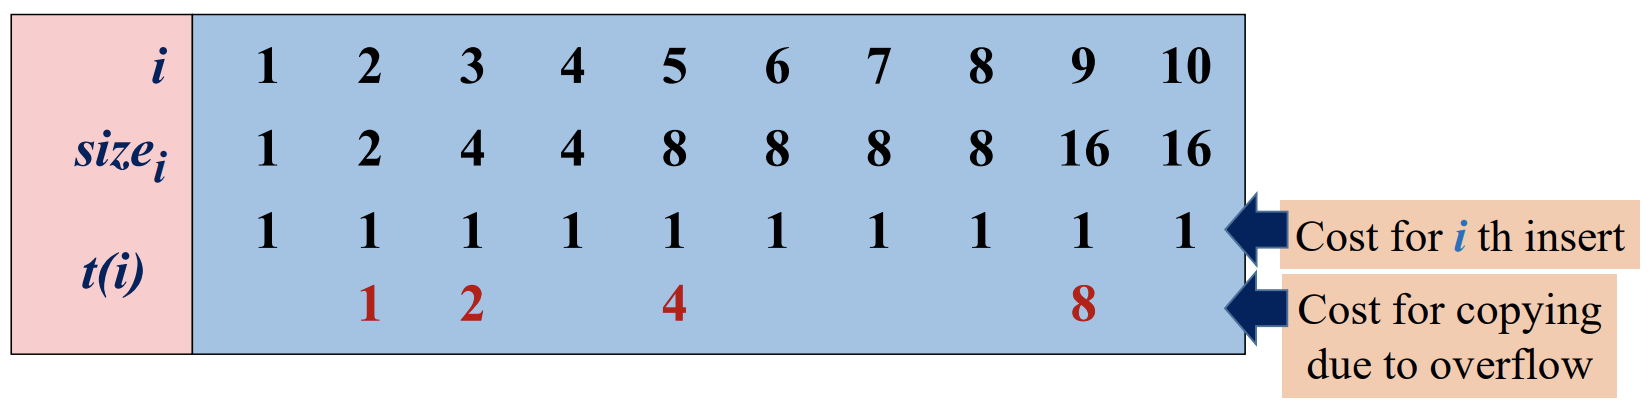
\includegraphics[width=0.95\linewidth]{st2131-dynamic-table-aggregate-method.png} 
  \end{tightcenter}

  \textbf{Accounting method}

  \begin{itemize}
    \item charge \$3 per insertion
      \begin{itemize}
        \item \$1 for insertion itself
        \item \$1 for moving itself when the table expands
        \item \$1 for moving one of the existing items when the table expands
      \end{itemize}
  \end{itemize}

  \textbf{Potential method}

  \begin{tightcenter}
    let $\phi(i) = 2i - size(T)$
    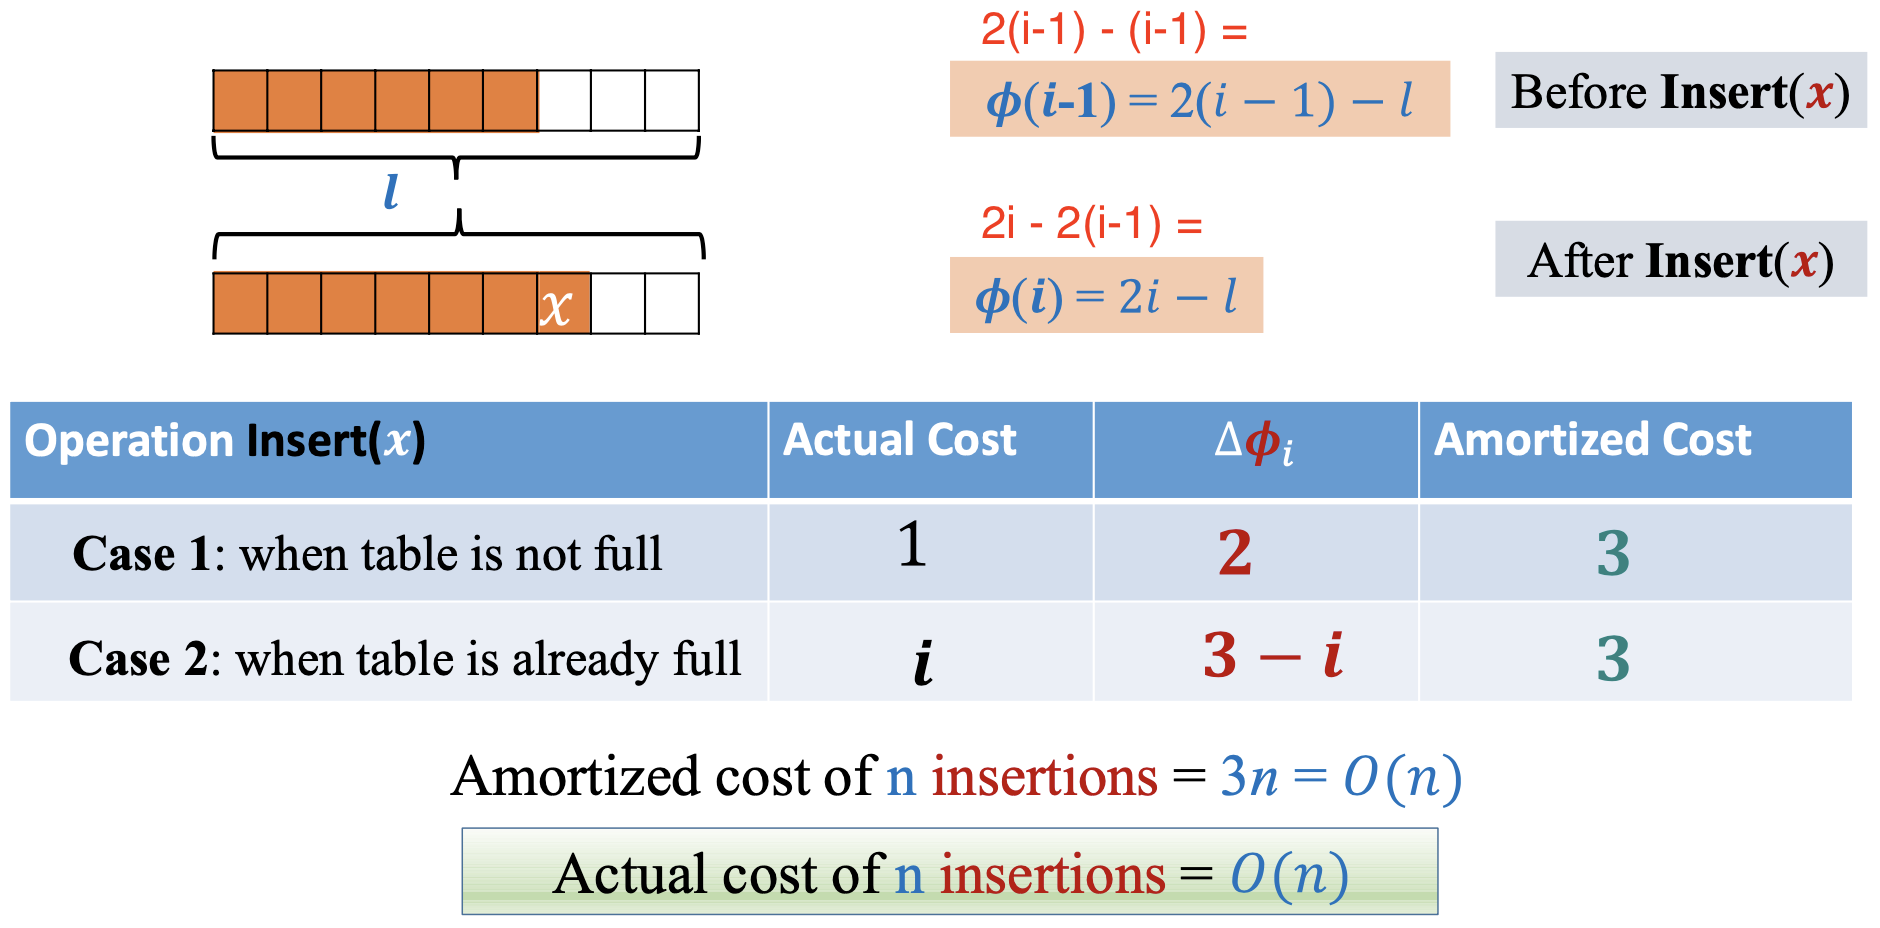
\includegraphics[width=0.95\linewidth]{st2131-dynamic-table-potential-method.png} 
  \end{tightcenter}
































\end{multicols*}

\pagebreak

\section{helpful approximations}

stirling's approximation: $T(n) = \sum\limits^n_{i=0} \log (n-i) = \log \prod^n_{i=0} (n-i) = \Theta(n \log n)$

harmonic number, $ H_n = \sum\limits_{k=1}^n \frac{1}{k} = \Theta(\lg n) $

basel problem: $\sum\limits^N_{n=1} \frac{1}{n^2} \leq 2 - \frac{1}{N} \xrightarrow{ N \to \infty } 2 $

$\quad\quad$ because $\sum^N_{n=1} \frac{1}{N^2} \leq 1 + \sum^{\log_3 n}_{x=2} \frac{1}{(x-1)x} = 1 + \sum^N_{n=2} (\frac{1}{n-1} - \frac{1}{n}) = 1 + 1 - \frac{1}{N} = 2 - \frac{1}{N} $

number of primes in range $\{1, \dots, K\}$ is $> \frac{K}{\ln K} $

\section{asymptotic bounds}

$1 < \log n < \sqrt{n} < n < n \log n < n^2 < n^3 < 2^n < 2^{2n}$

$\log_a n < n^a < a^n < n! < n^n$

for any $a, b > 0$, $\quad \log_a n < n^b$

\subsubsection{multiple parameters}

for two functions $f(m, n)$ and $g(m,n)$, we say that $f(m, n) = O(g(m, n))$ if there exists constants $c, m_0, n _0$ such that $0 \leq f(m,n) \leq c \cdot g(m,n)$ for all $m \geq m_0$ or $n \geq n_0$.

\subsection{set notation}

\begin{itemize}
  \item $O(g(n)) = \{f(n): \exists c, n_0>0 \mid \forall n \geq n_0, \, 0 \leq f(n) \leq cg(n)\}$
  \item $\Omega(g(n)) = \{f(n): \exists c, n_0>0 \mid \forall n \geq n_0, \, 0 \leq cg(n) \leq f(n)\}$
  \item $\Theta(g(n)) = \{ f(n): \exists c_1, c_2, n_0 > 0 \mid \forall n \geq n_0, \quad 0 \leq c_1 \cdot g(n) \leq f(n) \leq c_2 \cdot g(n) \}$ 
    $= O(g(n)) \cap \Omega(g(n))$
  \item $o(g(n)) = \{ f(n): \forall c > 0, \exists n_0 > 0 \mid \forall n \geq n_0, \quad 0 \leq f(n) < cg(n) \}$
  \item $\omega(g(n)) = \{ f(n) : \forall c > 0, \exists n_0 > 0 \mid \forall n \geq n_0, \quad 0 \leq cg(n) < f(n) \} $
\end{itemize}

\subsection{example proofs}

\begin{niceproof}
  that $2n^2 = O(n^3)$ 
  \\* let $f(n) = 2n^2$. then $f(n) = 2n^2 \leq n^3$ when $n \geq 2$. 
  \\* set  $c=1$ and $n_0 = 2$.
  \\* we have $f(n) = 2n^2 \leq c \cdot n^3$ for $n \geq n_0$. \qed
\end{niceproof}

\begin{niceproof}
  $n=o(n^2)$ 

  For any $c>0$, use $n_0 = 2/c$.
\end{niceproof}

\begin{niceproof}
  $n^2 - n =\omega(n)$ 

  For any $c>0$, use $n_0 = 2(c+1)$.
\end{niceproof}

\begin{niceproof}[Example]
  let $f(n) = n$ and $g(n) = n^{1 + \sin (n)}$. 

  Because of the oscillating behaviour of the sine function, there is no $n_0$ for which $f$ dominates $g$ or vice versa.

  Hence, we cannot compare $f$ and $g$ using asymptotic notation.
\end{niceproof}

\begin{niceproof}[Example]
  let $f(n) = n$ and $g(n) = n(2+\sin(n))$.

  Since $\frac{1}{3}g(n) \leq f(n) \leq g(n)$ for all $n \geq 0$, then $f(n) = \Theta(g(n))$.
  (note that limit rules will not work here)
\end{niceproof}

\section{mentioned algorithms}

\begin{itemize}
  \item ch.3 - \textbf{Misra Gries} - space-efficient computation of the majority bit in array $A$
  \item ch.3 - \textbf{Euclidean} - efficient computation of GCD of two integers
  \item ch.3 - \textbf{Tower of Hanoi} - $T(n) = 2^n-1$
    \begin{enumerate}
      \item move the top $n-1$ discs from the first to the second peg using the third as temporary storage. 
      \item move the biggest disc directly to the empty third peg.
      \item move the $n-1$ discs from the second peg to the third using the first peg for temporary storage.
    \end{enumerate}
  \item ch.3 - \textbf{MergeSort} - $T(n) = T(\lfloor n/2 \rfloor) + T(\lceil n/2 \rceil) + \Theta(n)$
  \item ch.3 - \textbf{Karatsuba Multiplication} - multiply two $n$-digit numbers $x$ and $y$ in $O(n^{\log_23})$
    \begin{itemize}
      \item worst-case runtime: $T(n) = 3T( \lceil n/2 \rceil ) + \Theta(n) $
    \end{itemize}
\end{itemize}

\section{uncommon notations}

\begin{itemize}
  \item $\bot$ - false
\end{itemize}

\end{document}
